\documentclass{article}
%encoding
%--------------------------------------
\usepackage[utf8]{inputenc}
\usepackage[T1]{fontenc}
%--------------------------------------
 
%German-specific commands
%--------------------------------------
\usepackage[ngerman]{babel}
\usepackage{csquotes}
%--------------------------------------
 
%Pictures
%--------------------------------------
\usepackage{graphicx}
\graphicspath{ {./Pictures/} }
\usepackage{tikz}
\usepackage{subcaption}
\usepackage{float}
\usepackage{wrapfig}
%--------------------------------------

%math
%--------------------------------------
\usepackage{amsmath}
\usepackage{amssymb}
\usepackage{amsfonts}
%--------------------------------------

%Frames
%--------------------------------------
\usepackage{framed}

%Own math commands
%--------------------------------------
\newcommand{\abs}[1]{\lvert#1\rvert}

%Colors
%--------------------------------------
\usepackage{xcolor}
\definecolor{blue-violet}{rgb}{0.54, 0.17, 0.89}
\definecolor{codegreen}{rgb}{0,0.6,0}
\definecolor{codegray}{rgb}{0.5,0.5,0.5}
\definecolor{codepurple}{rgb}{0.58,0,0.82}
\definecolor{backcolour}{rgb}{0.95,0.95,0.92}

%--------------------------------------
\usepackage{multicol}
%\usepackage{paracol}
%\usepackage[shortlabels]{enumitem}

%Aufgaben
%--------------------------------------
\usepackage{amsthm}
\newtheorem{aufgabe}{Aufgabe}[section]
\newtheorem{definition}{Definition}[section]
\newtheorem{beispiel}{Beispiel}[section]
%--------------------------------------

%Listings
%--------------------------------------
\usepackage{ulem}
\usepackage{listings}
 
\lstdefinestyle{mystyle}{
    backgroundcolor=\color{backcolour},   
    commentstyle=\color{codegreen},
    keywordstyle=\color{magenta},
    numberstyle=\tiny\color{codegray},
    stringstyle=\color{codepurple},
    basicstyle=\ttfamily\footnotesize,
    breakatwhitespace=false,         
    breaklines=true,                 
    captionpos=b,                    
    keepspaces=true,                 
    numbers=left,                    
    numbersep=5pt,                  
    showspaces=false,                
    showstringspaces=false,
    showtabs=false,                  
    tabsize=2,
    language=Python,
    morekeywords={repeat},
}
 
\lstset{style=mystyle,moredelim=[is][\sout]{|}{|}}
%--------------------------------------



\title{Funktionen in Tiger Jython - Konzeption}
\author{Alexandra Maximova}
\date{3. November 2020}

\begin{document}

\maketitle
\section{Rahmenbedingungen und Vorwissen}
Diese Lektion wird im Rahmen vom Einführungspraktikum an der Kantonsschule Menzingen zwei Mal in unterschiedlichen Halbklassen gehalten. Die SuS absolvieren das erste Jahr am Kurzzeitgymnasium und besuchen das OFI.

In den vorherigen Wochen haben die SuS angefangen, in Tyger Jython zu programmieren, und kennen schon viele Turtle-Befehle, Variablen und Schleifen. In dieser Lektion geht es darum, Funktionen einzuführen.

\section{Stoffanalyse}
\begin{figure}[H]
\centering
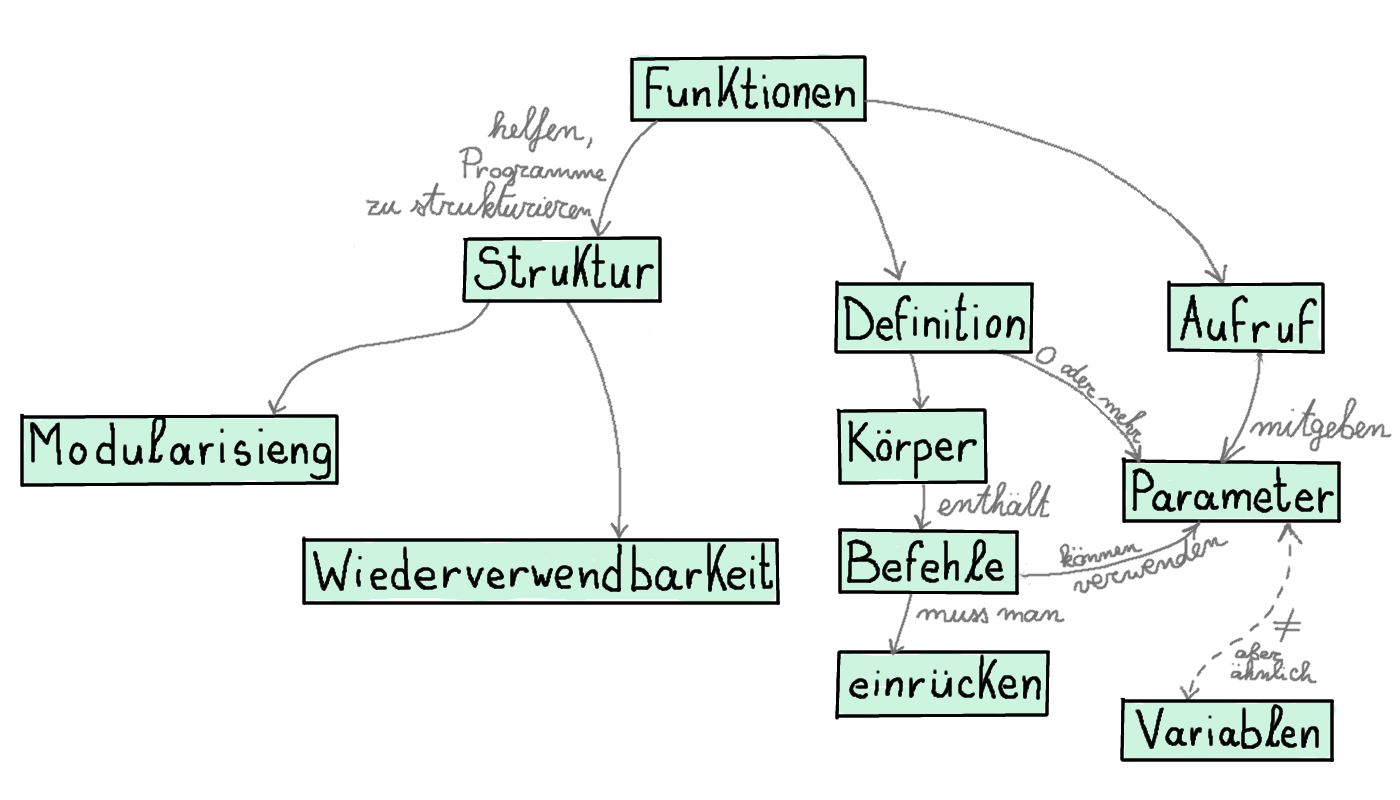
\includegraphics[width=\linewidth]{pictures/ConceptMap.png}
\end{figure}

\textbf{Funktionen} dienen dazu, den Code zu \textbf{strukturieren}. Sie fördern die \textbf{Modularisierung}, d.h. die Aufteilung in logischen \textbf{wiederverwendbaren} Bausteinen.

\textbf{Funktionen} muss man \textbf{definieren} und dann kann man sie beliebig oft \textbf{aufrufen}. In der \textbf{Definition} gibt man die Signatur und den \textbf{Körper} an. Zu der Signatur gehören der Name der Funktion und die \textbf{Parameter}. Im Körper stehen die \textbf{Befehle}, die ausgeführt werden, wenn die Funktion aufgerufen wird. Alle Befehle, die zu einer Funktion gehören, müssen in Tiger Jython \textbf{eingerückt} sein.

Beim \textbf{Funktionsaufruf} muss man den Namen der Funktion kennen und alle Parameter instanzieren.

Da der Begriff von \textbf{Parameter} und die Unterschiede zu den \textbf{Variablen} nicht selbstverständlich sind, empfiehlt es sich, zuerst \textbf{Funktionen ohne Parameter} einzuführen, und erst in der zweiten Stunde mit \textbf{Funktionen mit Parameter} fortzufahren.

\section{Lernziele}

\paragraph{Leitidee}
Digitale Medien und Technologien sind zum Alltag geworden. Damit die Erwachsenen von morgen diese neue Welt nicht nur konsumieren, sondern auch mitgestalten können, müssen die SuS von heute die Werkzeuge und die grundlegenden Konzepte kennenlernen. Programmieren und vor allem Modularisierung gehören dazu.

Das modulare Vorgehen, welches mit der Einführung von Funktionen trainiert wird, kann auch in anderen Situationen angewendet werden. Die SuS sollten lernen bei Projekten und Aufgaben Teile zu erkennen, die sie als Bausteine wiederverwenden können, um etwas Komplexeres zusammenzusetzen.

\paragraph{Dispositionsziele}
\begin{itemize}
\item Die SuS bevorzugen strukturierten Code.
\item Die SuS zerlegen Aufgaben in kleinere Teile, die als Module verwendet werden können.
\end{itemize}
\paragraph{Operationalisierte Lernziele}
\begin{itemize}
\item Die SuS definieren Funktionen ohne Parameter, die etwas Bestimmtes machen.
\item Die SuS rufen vor- oder selbstdefinierte Funktionen ohne Parameter auf.
\item Beim Zeichnen mit der Turtle, die SuS entscheiden selbstständig, welche Befehle sie in eine Funktion auslagern wollen, und rufen diese an den richtigen Stellen auf.
\item Die SuS definieren Funktionen mit Parameter, die etwas Bestimmtes machen.
\item Die SuS rufen vor- oder selbstdefinierte Funktionen mit Parameter auf, wobei sie für Parameter Zahlen einsetzen.
\item Die SuS rufen vor- oder selbstdefinierte Funktionen mit Parameter auf, wobei sie für Parameter Variablen einsetzen.
\end{itemize}


\section{Informativer Unterrichtseinstieg}
Wenn wir \lstinline|forward(25)| schreiben, geht die Schildkröte um 25 Schritte geradeaus. Wenn wir \lstinline|dot(25)| schreiben, zeichnet die Schildkröte einen Kreis mit Diameter 25. Wenn wir aber \lstinline|square()| schreiben, kommt eine Fehlermeldung.

Warum versteht die Schildkröte manche Befehle, und andere nicht? Können wir es ihr beibringen? Offensichtlich kann sie ein Quadrat zeichenen:

\begin{lstlisting}
repeat 4:
	forward(100)
	right(90)
\end{lstlisting}

Sie muss einfach verstehen, dass sie diese Befehle ausführen soll, wenn wir \lstinline|square()| schreiben.

Heute werden wir lernen, wie man in Tyger Jython dem Computer neue Befehle beibringt. Das nennen wir \textbf{Funktionen}. In der ersten Stunde befassen wir uns mit einfachen Befehlen. Ihr werdet Zeit haben, selbstständig 4 Aufgaben zu lösen. Nach der Pause werden wir sehen, wie wir mehrere leicht unterschiedliche Befehle auf einmal definieren können.

Nach der Stunde wird jeder von euch der Schildkröte neue Befehle beibringen können und den Code besser strukturieren.

Warum wollen wir überhaupt neue Wörter der Schildkröte beibringen? Wir können doch alles mit den Grundbefehlen penUp, penDown, forward, right zeichnen.
Wenn die Formen aber komplexer werden, sehnen wir uns nach Struktur. Wenn wir ein Haus zeichnen, zeichnen wir das Haus, das Dach, die Tür, die Fenster usw. Wir können aus einfachen Formen kompliziertere bauen, und diese wiederum wiederverwenden, um noch etwas grösseres und komplexeres zu bauen. (Das gilt, übrigens, nicht nur für Zeichnungen mit der Schildkröte, sondern auch für Berechnungen und Computerspiele).

Angenommen, wir wollen der Schildkröte beibringen, was ein Quadrat ist. Dafür definieren wir in Tiger Jython eine Funktion \lstinline|square()|. Wir wissen, was sie machen muss.
\begin{lstlisting}
def square():
	repeat 4:
		forward(100)
		right(90)
\end{lstlisting}
Das Keyword \lstinline|def| macht die Schildkröte aufmerksam, dass sie die Definition eines neuen Befehls sieht. Nach dem Keyword kommt der \textbf{Name} der Funktion. Es ist frei wählbar, wie der Name einer Variable, und es empfiehlt sich, einen Namen zu wählen, welcher beschreibt, was die Funktion machen soll. In diesem Fall haben wir die Funktion \lstinline|square| genannt, weil sie ein Quadrat zeichnen soll.

Diese Funktion, die wir gerade definiert haben, können wir \textbf{aufrufen}, d.h. verwenden, um andere Figuren zu zeichnen.
Zum Beispiel, können wir aus Quadrate Tetris-Figuren zeichnen:
\begin{multicols}{2}
\begin{lstlisting}
from gturtle import *

def square():
    repeat 4:
        forward(100)
        right(90)
        

makeTurtle()

square()
forward(100)
square()
right(90)
forward(100)
left(90)
square()
forward(100)
square()
\end{lstlisting}
\columnbreak
\begin{figure}[H]
\centering
\includegraphics[width=\linewidth]{pictures/tetris.png}
\end{figure}
\end{multicols}



\section{Literatur}
Für die Erstellung von Skript und Aufgaben wurden das Skript von Tobias Kohn (zu finden auf https://tobiaskohn.ch/index.php/teaching/teaching-python/) und der Kurs 2 der Begabtenförderung (verfügbar auf Moodle) verwendet.

\end{document}